\subsection{\label{subsec:FZV3}Absorption}
\textbf{\textit{a) Erläutern Sie das übliche Absorptionsgesetz für die Schwächung monochromatischer
Strahlung beim Durchgang durch Materie!}}\\
$\rightarrow$Das Absorptionsgesetz beschreibt, wie die Intensität der Röntgenstrahlung 
beim Durchgang durch Materie abnimmt. Das Gesetz basiert auf der Wechselwirkung der Strahlung mit den Atomen 
oder Molekülen in der Materie. Das übliche Absorptionsgesetz wird oft als das sogenannte Beer-Lambert-Gesetz
bezeichnet und kann folgendermaßen ausgedrückt werden \cite{Kristall}
\begin{align}
    I(x) &= I_{0}e^{-\mu_{\text{ges,M}}\rho x} \\
    \mu_{\text{ges,M}} &= \frac{\mu_{\text{ges}}}{\rho} \\
    \mu_{\text{ges}} &= \mu_{\text{abs}} + \mu_{\text{ray}} + \mu_{\text{com}} + \mu_{\text{ppn}} + \mu_{\text{ppe}}.
\end{align}
Hierbei steht $I(x)$ für die Intensität des Strahls, nach Durchgang einer Probe der Dicke $x$, $I_{0}$ entspricht der
Anfangsintensität, $\rho$ der Probendichte und $\mu_{\text{ges,M}}$ ist der gesamte Massenschwächungskoeffizient, 
welcher sich als Quotient aus dem Absorptionskoeffizienten $\mu$ und der Dichte $\rho$ ergibt. 
Wie in der vorherigen Frage erläutert spielen verschiedene Wechselwirkungen der Strahlung mit Materie eine Rolle, die 
jeweils zur Schwächung der Intensität führen. Die verschiedenen Beiträge beruhen auf Photoabsorption $\mu_{\text{abs}}$, 
kohärenten Rayleigh-Streuung $\mu_{\text{ray}}$, inkohärenten Compton-Streuung $\mu_{\text{com}}$ und der 
Paarbildung im Coulombfeld des Kerns $\mu_{\text{ppn}}$ bzw.~des Elektrons $\mu_{\text{ppe}}$.
Diese Beiträge sind in Abb.~\ref{fig:absorp} zusammengefasst dargestellt, wobei erkennbar ist, dass 
die Paarbildung erst bei sehr hohen Energien eine Rolle spielt.
\begin{figure}[h!]
    \centering
    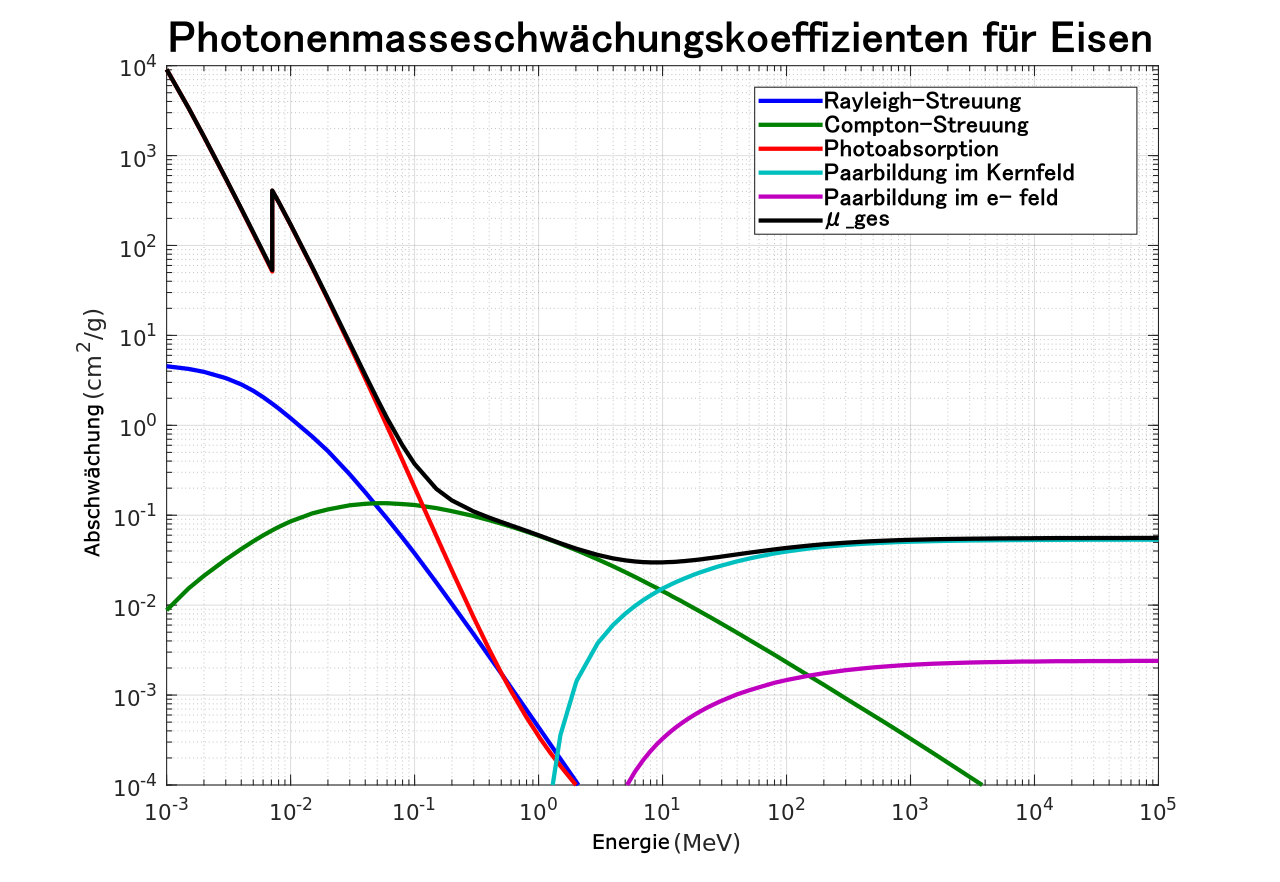
\includegraphics[width=0.45\textwidth]{Absorp.png}
    \caption{\label{fig:absorp}Einzelbeiträge zum, sowie gesamter Massenschwächungskoeffizient
    als Funktion der Energie für das Beispielmaterial Eisen. Die einzelnen Beiträge sind der Legende zu 
    entnehmen und im Haupttext erläutert. Die Graphik wurde aus Ref.~\cite{Absorp} entnommen.}
\end{figure} \FloatBarrier \,\\
Zusammenfasst sagt das Beer-Lambert-Gesetz aus, dass die Intensität der Strahlung exponentiell mit der Dicke der 
durchquerten Materieschicht abnimmt. Je größer der Absorptionskoeffizient, desto schneller nimmt die Intensität ab, 
wobei $\mu$ von der Art der Strahlung und der durchstrahlten Materie abhängt. \\

\textbf{\textit{b) Warum entstehen die Absorptionskanten?}}\\
$\rightarrow$Ein Röntgenquant kann ein Elektron aus einem gebundenen Zustand im Atom nur dann herauslösen, 
wenn die Energie ausreicht, um das Elektron in einen unbesetzten Zustand zu versetzen oder komplett aus der Bindung zu lösen. 
Bei schrittweiser Erhöhung der Röntgenstrahlungsenergie erfolgt ein abrupter Anstieg der Röntgenabsorption des Materials, 
sobald der Punkt erreicht ist, an dem dieser Prozess möglich wird. 
Dieser markante Anstieg wird als Absorptionskante bezeichnet, wobei die Absorption in ihrer Nähe von der 
Verfügbarkeit unbesetzter Zustände einer spezifischen Energie für das Elektron abhängt \cite{Demtroder}. \\

\textbf{\textit{c) Skizzieren Sie für ein bestimmtes Element den Verlauf des Schwächungskoeffizienten 
$\mu$ als Funktion der Energie, $\mu(E)$, bzw. der Wellenlänge, $\mu(\lambda)$!}}\\
$\rightarrow$Die in Abb.~\ref{fig:daten} dargestellten Daten wurden aus Ref.~\cite{Tabe} entnommen und für Blei (Pb) einerseits 
mit dessen Dichte multipliziert und als Funktion der Wellenlänge umgerechnet. 
\begin{figure}[h!]
    \centering
    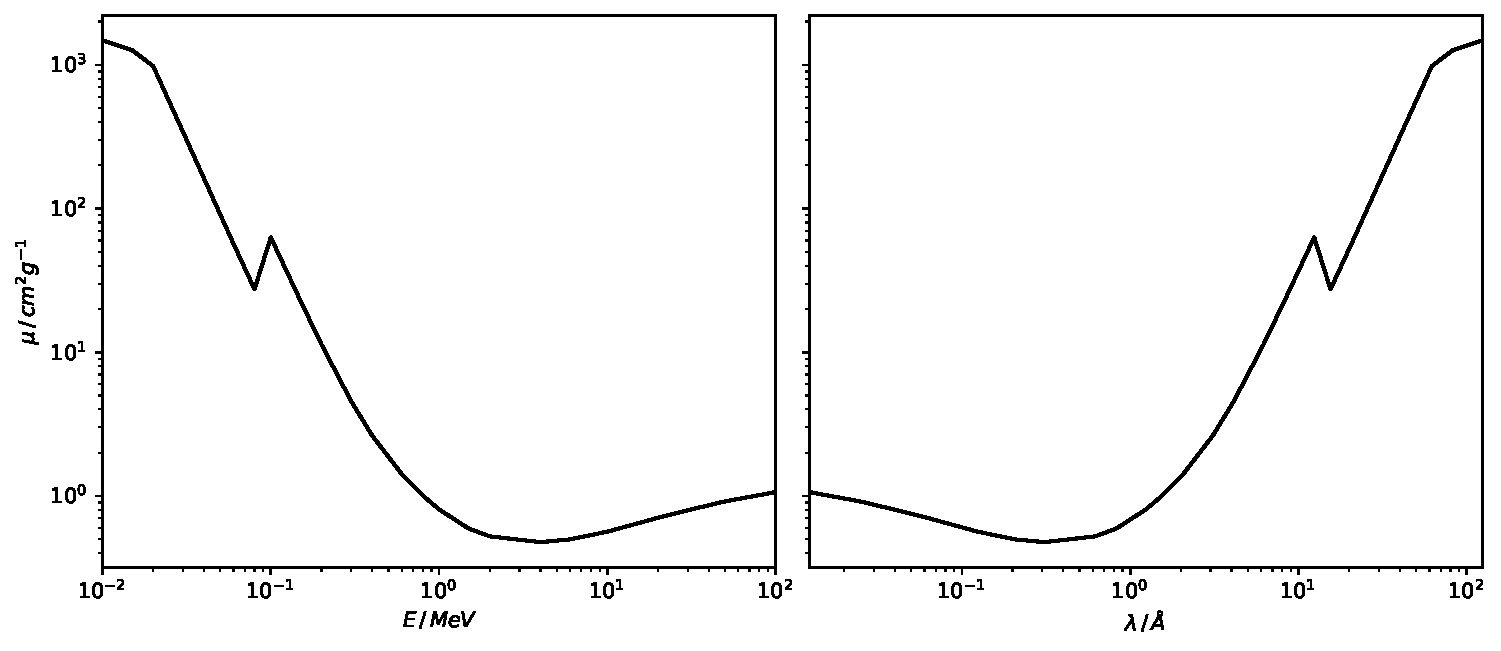
\includegraphics[width=0.8\textwidth]{skizze.pdf}
    \caption{\label{fig:daten}Der Schwächungskoeffizient $\mu$ für Blei als Funktion der Energie (links) und der 
    Wellenlänge (rechts). Aufgrund der logarithmischen Darstellung unterscheiden sich die Datensätze kaum ($\log(hc/E)=\log(hc) - \log(E)$).
    Die deutlich erkennbare K-Absorptionskante liegt bei $88\,\si{keV}$.}
\end{figure}\FloatBarrier 